\subsubsection{Projekt hinzufügen}
\begin{figure}[H]
  \begin{center}
    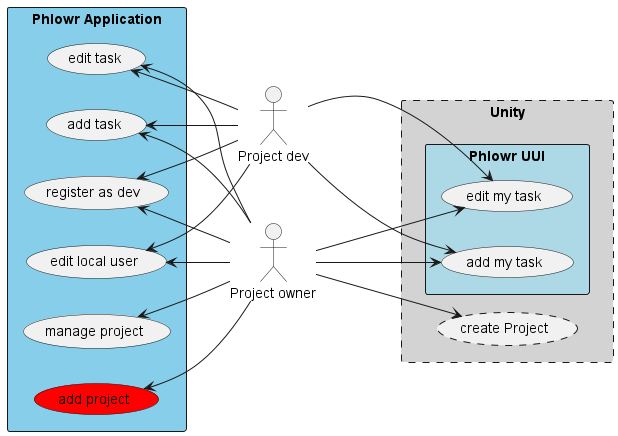
\includegraphics[width=0.3\linewidth]{../content/diagrams/usecase/overview/overviewUseCaseAddProjectSelected.png}
    \caption{Use Case Diagaramm <add project> }
  \end{center}
\end{figure}


\begin{table}[H]
    \centering
    \settowidth\tymin{executeIncomingCommand()}
    \setlength\extrarowheight{2pt}
    \begin{tabulary}{1.0\textwidth}{|m{4cm}|m{10cm}|}
      \hline
      \textbf{Use Case} &
      \textbf{ADD PROJECT}\\
      \hline
      \textbf{Beschreibung} &
      Ein Unity-Projekt wird der Applikation hinzugefügt\\ 
      \hline
      \textbf{Includes} &
      \begin{itemize}
        \item keine 
      \end{itemize}\\ 
      \hline
      \textbf{Akteure} &
      \begin{itemize}
        \item Project Owner
      \end{itemize}\\ 
      \hline
      \textbf{Auslöser} &
      \begin{itemize}
        \item Ein bestehendes Unity-Projekt soll mit Phlowr verwaltet werden
      \end{itemize}\\ 
      \hline
      \textbf{Vorbedingungen} &
      \begin{itemize}
        \item Das hinzuzufügende Unity-Projekt wurde bereits erstellt
      \end{itemize}\\ 
      \hline
      \textbf{Abschlussbedingungen} &
      \begin{itemize}
        \item Das gewünschte Projekt ist in der Applikation erfasst
      \end{itemize}\\ 
      \hline
      \textbf{Ablauf} &
      \begin{enumerate}
        \item Applikation öffnen
        \item <Projekt Hinzufügen> wählen
        \item Den entsprechenden Projekt-Ordner auswählen
        \item Speichern
        \end{enumerate}\\ 
      \hline
      \textbf{Zu Beachten / Notizen} &
      \begin{itemize}
        \item Projekt sollte nur einmal hinzugefügt werden können
        \item Projekt Ordner-Struktur sollte überprüft werden
        \end{itemize}\\ 
      \hline
    \end{tabulary}
    \caption{Use Case: ADD PROJECT}
  \end{table}
